\documentclass[aspectratio=169]{beamer}
\usepackage[utf8]{inputenc}
\usepackage[german]{babel}
\usepackage{graphics}
\usepackage{amsmath}

\usetheme{Berlin}

\title{Korrektheit von Programmen beweisen mit Coq}
\institute{Linux Tag Tübingen 2016}
\author{Peter Hrenka}
\date{\today}

\begin{document}
\begin{frame}
\titlepage
\end{frame}
\section*{Übersicht}
\begin{frame}
  \tableofcontents
\end{frame}
\begin{frame}
  \frametitle{Über mich}
  \begin{itemize}
    \item Linux Anwender seit 1995
    \item Studium Informatik und Mathematik in Tübingen
    \item Sofwareentwickler \texttt{C++}, \texttt{python}, OpenGL
  \end{itemize}
\end{frame}
\section{Einführung}
\subsection{Softwarequalität}
\begin{frame}
  \begin{center}
    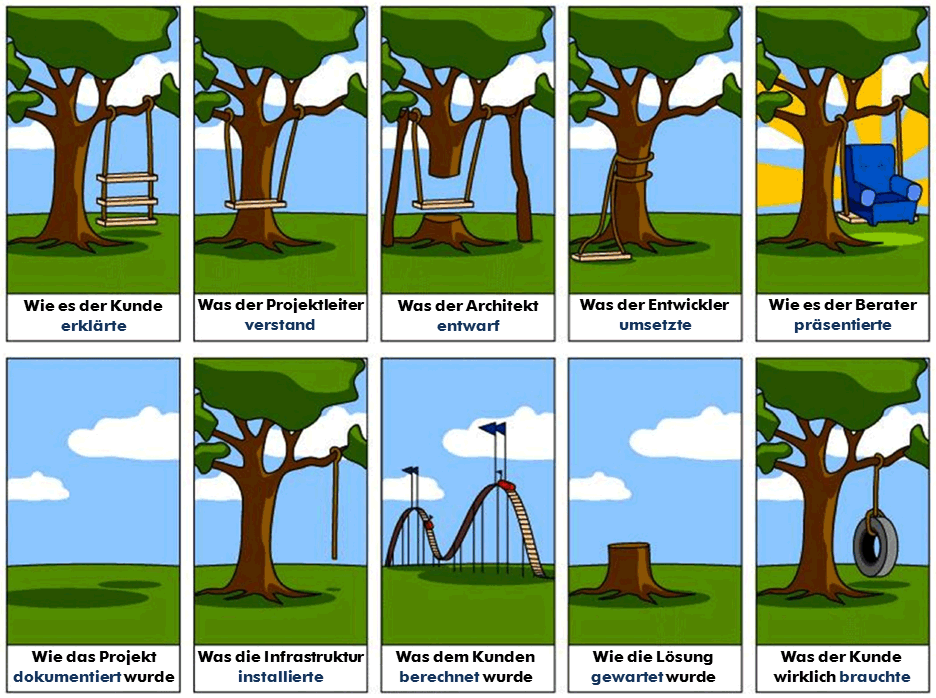
\includegraphics[width=9.2cm]{projekt-schaukel-baum.png}
  \end{center}
\end{frame}
\begin{frame}
  ``Jedes nicht-triviale Programm hat Fehler''\\
  \pause
  \vfill
  Warum?
  \pause
  \vfill
  \begin{enumerate}
    \item Fehlendes Verständnis des Problems
    \pause
    \item Fehlerhafte ``Spezifikation''
    \pause
    \item Implementierung nicht korrekt
  \end{enumerate}
\end{frame}
\subsection{Methoden}
\begin{frame}
  Wie kann man die Korrektheit (bzgl. der Spezifikation) sicherstellen?
  \vfill
  \begin{itemize}
  \item Testen
  \item Pair Programming
  \item Code Reviews
  \item Bug Bounties
  \item Open Source
  \item Statische Analyse \pause
  \end{itemize}
  \vfill
  \begin{center}
    Reicht das? 
  \end{center}
\end{frame}
\begin{frame}
  \begin{center}
    \Large{Timsort}
  \end{center}
  \begin{itemize}
  \item Verbreiteter Sortieralgorithmus (Java, Android)
  \item relativ kompliziert
  \item 2015: Formale Verfikation fehlgeschlagen! $\rightarrow$ Bug!
  \item \href{http://envisage-project.eu/proving-android-java-and-python-sorting-algorithm-is-broken-and-how-to-fix-it/}{proving-android-java-and-python-sorting-algorithm-is-broken}
  \item Verwendetes Tool KeY: \url{http://www.key-project.org/}
  \end{itemize}
\end{frame}
\begin{frame}
  \begin{center}
    
\includegraphics[width=4.0cm]{sel4_logo.pdf}
    \Large{\texttt{seL4}}
  \end{center}
  \begin{itemize}
  \item Microkernel, Devices laufen im Userspace
  \item Implementiert in C
  \item Läuft auf ARM, x86
  \item GPL
  \item Formaler Beweis mit Beweisassistenzsystem \texttt{Isabelle/HOL}
    \begin{itemize}
    \item Keine Pufferüberläufe, Null-Pointer-Zugriffe oder use-after-free
    \item Code erfüllt die Spezifikation, Sicherheitsaspekte
    \item Binärcode ebenfalls verifiziert (Compiler hat keine Fehler gemacht)
    \end{itemize}
  \end{itemize}
\end{frame}
\begin{frame}
  \begin{center}
    \Large{Wie soll so ein Beweis funktionieren?}
  \end{center}
  \pause
  \vfill
  \begin{center}
    \Large{Macht das Spaß?}
  \end{center}  
\end{frame}
\section{Coq}
\begin{frame}
  \begin{center}
    
\includegraphics[width=1.0cm]{coq_logo.png}
    \Large{\texttt{Coq}}
  \end{center}
  \begin{itemize}
  \item Beweisassistenzsystem
  \item ``coq'': französisch ``Hahn''
  \item entwickelt am INRIA
  \item implementiert in \texttt{OCaml}
  \item verwendet ``dependent types''
  \item interaktiv, eigene IDE \texttt{coqide} oder \texttt{Proof General} für Emacs
  \item online (via JS transpiler) \url{https://x80.org/rhino-coq/}
  \end{itemize}
\end{frame}
\begin{frame}
  \begin{center}
    \Large{Mathematik mit \texttt{Coq}}
  \end{center}
  \begin{itemize}
  \item Vier-Farben-Satz, 2005
  \item Satz von Feit-Thomson (Gruppentheorie), 2012
  \item Univalent Foundations, Homotopy Type Theory (HoTT), ca. 2012
  \end{itemize}
  \pause
  \vfill
  \begin{center}  
    $\rightarrow$ scheint für Mathematik brauchbar, wie sieht es mit Informatik aus?
  \end{center}
\end{frame}
\begin{frame}
  \begin{center}
    \Large{CompCert}
  \end{center}
  \begin{itemize}
  \item ``Compilers you can \textit{formally} trust''
  \item große Teilmenge von ISO C90 / ANSI C
  \item MISRA-C 2004
  \item generiert effizienten Code für PowerPC, ARM and x86\\
    ``about 90\% of the performance of GCC version 4 at optimization level 1''
  \item implementiert in \texttt{OCaml} und \texttt{coq}
  \item geleitet von Xavier Leroy (LinuxThreads) 
  \item nicht-freie Lizenz, aber einige Teile unter GPL und BSD
  \end{itemize}
\end{frame}
\begin{frame}
  \begin{center}
    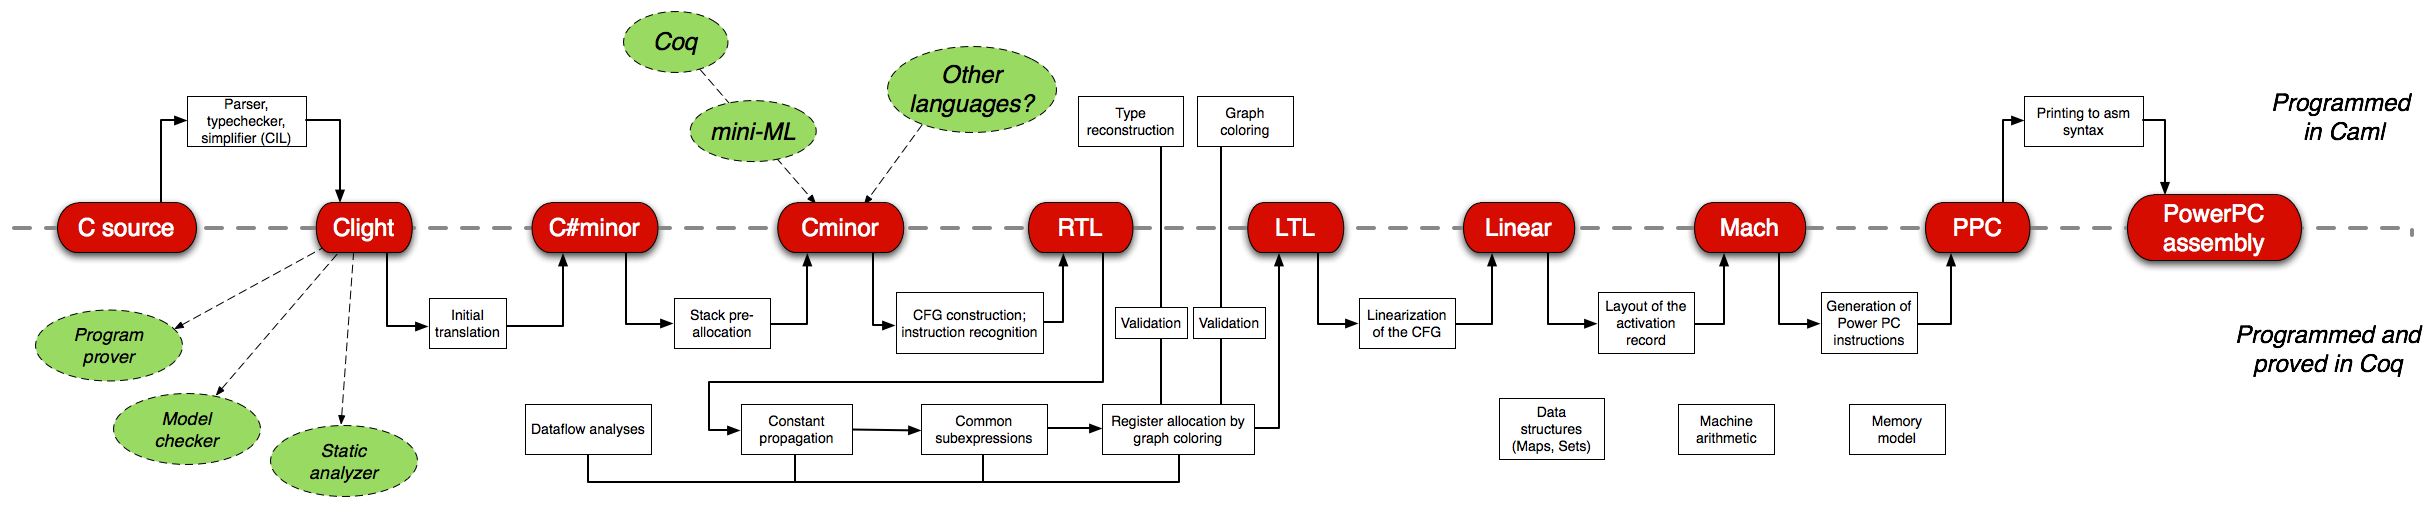
\includegraphics[width=20.0cm]{compcert_diagram.png}
  \end{center}
\end{frame}
\begin{frame}
  \begin{center}
    %
\includegraphics[width=3.0cm]{why3_logo.png}    
    \Large{\texttt{Why3}}
  \end{center}
  \begin{itemize}
  \item Platform für Programmverfikation von Programmen in \texttt{WhyML}
  \item Anbindungen für andere Programmiersprachen existieren
    \begin{itemize}
    \item \texttt{Frama-C} für \texttt{C}
    \item \texttt{SPARK} für \texttt{Ada}
    \end{itemize}
  \item Automatische Solver: \texttt{Alt-Ergo}, \texttt{CVC3/4}, \texttt{Z3}, uvm. 
  \item Manuelle Solver: \underline{\texttt{coq}}, \texttt{PVS} und \texttt{Isabelle/HOL}
  \end{itemize}
\end{frame}
\begin{frame}
  \begin{center}
    
\includegraphics[width=8.0cm]{spark_logo.jpg}    
    %\Large{\texttt{SPARK}}
  \end{center}
  \begin{itemize}
  \item Erweitere Untermenge von \texttt{Ada}
  \item kann Vor- und Nachbedingungen teilweise zur Compilezeit prüfen
  \item kann \texttt{coq}-Code exportieren, um schwere Fälle manuell zu beweisen
  \item Pro- und GPL Editionen
  \end{itemize}
\end{frame}
\begin{frame}
  \begin{center}
    
\includegraphics[width=3.0cm]{fscq_logo.png}
  \end{center}
  \begin{itemize}
  \item ``A Formally Certified Crash-proof File System''
  \item Nachweis, daß bei Absturz zu beliebigem Zeitpunkt keine Daten verloren gehen
  \item MIT 2015, u.A. Adam Chlipala
  \item implementiert und verfiziert in \texttt{coq}
  \item extrahierbar nach \texttt{ocaml}, \texttt{Haskell} oder \texttt{go}
  \item verwenbar mit \texttt{fuse} 
  \end{itemize}
\end{frame}
\section{Demo}
\begin{frame}
  \begin{center}
    \huge{Demo}
  \end{center}
\end{frame}
\section{Fazit}
\begin{frame}
  \begin{center}
    \Large{Demo hat gezeigt}
  \end{center}
  \begin{itemize}
  \item Aussagenlogik ist leicht
  \item Arithmetik ist fummelig
  \item Coq $=$ schlechtestes Taschenrechnerprogramm der Welt!
  \item Sätze sind Typen, Programme sind Beweise (Curry-Howard-Isomorphismus)
  \item Induktion geht nicht nur mit $n\in\mathbb{N}$
  \item Automatisierung hilft
  \end{itemize}
\end{frame}
\begin{frame}
  \begin{center}
    \Large{Dokumentation}
  \end{center}
  \begin{itemize}
  \item gutes Tutorial zum Durcharbeiten: Software Foundations\\
    \qquad \url{http://www.cis.upenn.edu/~bcpierce/sf/current/index.html}
  \item Älteres Buch: Interactive Theorem Proving and Program Development
  \item Online-Buch (Fortgeschritten): Certified Programming with dependent types:\\
    \qquad \url{http://adam.chlipala.net/cpdt/}
  \item Offizielle Doku:\\
    \qquad \url{https://coq.inria.fr/documentation}
  \end{itemize}
\end{frame}
\begin{frame}
  \begin{center}
    \Large{Probleme}
  \end{center}
  \begin{itemize}
  \item Offizielle Dokumentation (höchstens) zum Nachschlagen geeignet
  \item Standardbibliothek mathematiklastig, wenig Datenstrukturen
  \item Unidirektione Arbeitsweise 
    \begin{itemize}
    \item \texttt{coq} $\longrightarrow$ \texttt{OCaml}
    \end{itemize}
  \item Kein Export nach \texttt{C}, \texttt{C++}, $\left<\textit{mainstream Sprache}\right>$
  \end{itemize}
\end{frame} % to enforce entries in the table of contents
\begin{frame}
  \begin{center}
    \Large{Projekte}
  \end{center}
  \begin{itemize}
  \item Floats for Coq: formalisiere Fließkommazahlen\\
    \qquad \url{http://flocq.gforge.inria.fr/}
  \item JSCert: Coq specification of ECMAScript 5\\
    \qquad \url{https://github.com/jscert/jscert}
  \item The C11 standard formalized in Coq\\
    \qquad \url{http://robbertkrebbers.nl/thesis.html}
  \item RustBelt: Logical Foundations for the Future of Safe Systems Programming\\
    \qquad \url{http://plv.mpi-sws.org/rustbelt/}
  \end{itemize}
\end{frame}
\begin{frame}
  \begin{center}
    \Huge{Vielen Dank!}\\
    ~\\
    ~\\
    \Large{Fragen?}
  \end{center}
\end{frame}
\end{document}